% Ethical considerations: Consider any ethical issues related to 
% the use of the dataset, such as privacy concerns, bias, or limitations 
% in the data's representativeness.
\section{Zbiór danych}

Dane wykorzystane w doświadczeniach pochodzą ze zbioru ERA5 opublikowanego przez ECMWF.
Zbiór ten jest zbiorem reanalysis globalnej pogody pokrywający dane od 1940 roku do dziś.
ERA5 została stworzona przez Copernicus Climate Change Service (C3S) będącym częścią ECMWF.
ERA5 zapewnia godzinne estymaty wielu zmiennych pogodowych dotyczących warunków atmosferycznych,
oceanicznych oraz lądowych. Dane pokrywają ziemię siatką o rozdzielczości 30 km z wertykalnym podziałem
sięgającym 137 poziomów od powierzchni do 80 km. Dodatkową informacją w zbiorze danych są zmienne
opisujące niepewność pomiarową zawartych pomiarów. ERA5 udostępnia także dzienne i miesięczne 
statystyki obliczone na podstawie podstawowych pomiarów.

Ten zbiór wykorzystuje szeroką gamę obserwacji historycznych zebranych razem i przetworzonych
poprzez zaawansowane techniki asymilacji danych i modelowania numerycznego w celu uzyskania 
dokładnych estymatów globalnych.

Pomimo bogactwa informacji zaprezentowanego przez zbiór ERA5 posiada on także pewne 
ograniczenia, które muszą być wzięte pod uwagę podczas jego analizy. Z powodu zmian w systemie
obserwacyjnym niektóre zmiany nie są spowodowane z przyczyn fizycznych obserwowanego systemu.
Przykładem takiej zmiany może być wprowadzenie danych dotyczących zakrycia radiowego (ang.
radio occultation) w 2006 roku przez program COSMIC.
Co więcej, reprezentacja niektórych zmiennych klimatycznych takich jak przepływy energii
powierzchniowej mogą nie być wiarygodnie zaprezentowane.

Źródłami odczytów pomiarowych dla zbioru ERA5 były między innymi IASI, 
ASCAT, CrIS, MWHS, MWHS-2, TMI, SSMIS, AMSR-2, GMI będącymi zaawansowanymi urządzeniami
służącymi do pomiaru warunków atmosferycznych.

Chociaż zbiór ten udostępnia wyniki modeli ensemble, wnioskuje się, że niepewności 
prognozowanie są niedostatecznie  reprezentowane. Chociaż zbiór ten jest bardzo ważnym 
zasobem i kolejnym krokiem w stronę integralnego zbioru pogodowego, to spójność i 
dokładność globalnie uśrednionej temperatury w górnej stratosferze nie została polepszona
w stosunku do wcześniej upublicznionych zbiorów danych.

Zbiór danych ERA5 jest wciąż rozwijany, a miesięczne aktualizacje danych są mniej więcej
z dwumiesięcznym opóźnieniem.

% Data source: Explain where the data came from, whether it 
% was publicly available or collected specifically for your research. 
% If you used multiple sources, describe how you combined them and any 
% challenges you encountered.
\subsection{Źródło danych}

Dane wykorzystane w niniejszej pracy zostały pobrane z otwartego źródła, jakim jest
\href{https://cds.climate.copernicus.eu/cdsapp#!/dataset/reanalysis-era5-land?tab=form}{Copernicus Climate Change Service}.
Strona ta udostępnia ogólnodostępne API, dzięki któremu każdy użytkownik jest w stanie
wysłać zapytanie o interesujący go zakres danych. Dzięki temu API możliwe jest sprecyzowanie
przedziału czasowego, zakresu geograficznego oraz typów zmiennych. Przykładowe zapytanie jest 
zaprezentowane na następującym listingu \ref{json-listing}.

Strona Copernicus Climate Change Service posiada ponad 180 000 użytkowników z 171 krajów. Sumaryczna
ilość obsłużonych żądań danych przewyższa 519 milionów, a łączna ilość przesłanych danych wynosi
w przybliżeniu 125 petabajtów.

Darmowe konto narzuca jednak użytkownikowi limit wielkości danych możliwych do pobrania 
za pomocą jednego żądania API. W przypadku zbyt dużej ilości danych konieczne
jest wielorazowe wywołanie zapytania i następne złożenie danych.

\begin{lstlisting}[label=json-listing,caption={Przykładowe zapytanie API CDS Climate Copernicus},language=json]
{
    'variable': [
        '10m_u_component_of_wind', 
        '10m_v_component_of_wind', 
        '2m_temperature',
        'runoff', 
        'surface_net_solar_radiation', 
        'surface_net_thermal_radiation',
        'surface_pressure', 
        'total_evaporation', 
        'total_precipitation',
    ],
    'year': '2023',
    'month': '01',
    'day': '31',
    'time': [
        '00:00', '01:00', '02:00',
        '03:00', '04:00', '05:00',
        '06:00', '07:00', '08:00',
        '09:00', '10:00', '11:00',
        '12:00', '13:00', '14:00',
        '15:00', '16:00', '17:00',
        '18:00', '19:00', '20:00',
        '21:00', '22:00', '23:00',
    ],
    'area': [
        49.91, 18.89, 49.89,
        18.91,
    ],
    'format': 'netcdf.zip',
}
\end{lstlisting}

Otrzymane dane są w formacie NetCDF, będącym samo opisującym, niezależnym platformowo formatem
wyspecjalizowanym do tworzenia i udostępniania danych tablicowych. NetCDF jest otwartym standardem
stworzonym przez UCAR (University Corporation for Atmospheric Research). Istnieje wiele bibliotek
wspierających ten format, między innymi dostępne są także w języku Python \cite{python}.

% Data characteristics: Discuss the characteristics of the data, such as 
% its size, structure, and complexity. If your dataset includes multiple variables, 
% explain how you selected the variables of interest and any transformations you applied.
\subsection{Charakterystyka danych}

\subsubsection*{Wybrane zmienne}

\begin{itemize}
    \item Składowa pionowa i pozioma prędkości wiatru (u10, v10) — 
    Składowe skierowane w kierunku wschodnim i północnym zmierzone na wysokości 10 metrów nad poziomem
    morza i wyrażone w metrach na sekundę.

    \item Temperatura 2 metry nad poziomem ziemi (t2m) — Temperatura 2 metry nad poziomem ziemi jest
    obliczana, interpolując pomiędzy najmniejszym poziomem modelu oraz poziomem ziemi biorąc pod
    uwagę warunki atmosferyczne. Temperatura jest wyrażona w Kelwinach.

    \item Zmiany poziomów cieków wodnych (ro) — 
    Pewne ilości wody pochodzące z opadów, topnienia, lub z wód podziemnych pozostają w ziemi, lecz reszta
    odnajduję ujście poprzez cieki podziemne, bądź poprzez powierzchnię ziemi. Suma tych dwóch
    odpływów wody daje całkowitą wartość. Całkowita wartość jest zakumulowana z godzinnego
    okna analizy. Jednostką tej zmiennej jest głębokość opisująca głębokość ilości wody, jeśli byłaby
    równomiernie rozłożona na kilometr kwadratowy jednej komórki siatki. Ten wskaźnik jest
    bezpośrednio powiązany z dostępnością wody w glebie i może wskazywać na suszę bądź potopy.

    \item Promieniowanie słoneczne (ssr) — opisuje ilość promieniowania słonecznego (krótkofalowego), które dociera do 
    płaszczyzny ziemi (w sposób bezpośredni, jak i poprzez dyfuzję) pomniejszoną o ilość energii
    odbitej od powierzchni ziemi. Ta zmienna jest agregowana poprzez jedną godzinę i wyrażana w 
    dżulach na metr kwadratowy.

    \item Promieniowanie termiczne (str) — wielkość charakteryzująca ilość promieniowania termicznego
    (długofalowego) oddawanego przez ziemię w kierunku pionowym. Atmosfera oraz chmury emitują 
    promieniowanie w każdym kierunku, z czego pewna część dociera do powierzchni ziemi. Wartość
    tej zmiennej jest obliczona jako bilans energii oddawanej i otrzymywanej przez ziemię. 
    Promieniowanie jest akumulowane w godzinnym okresie i wyrażane w dżulach na metr kwadratowy.

    \item Ciśnienie (sp) — wyraża ciśnienie atmosferyczne na powierzchni ziemi bądź wody. Wielkość
    ta wyrażona została w pascalach. Duże zmiany ciśnienia razem ze wzrostem wysokości sprawiają,
    że trudno wyrazić wartość tej zmiennej ponad górzystymi terenami, więc często średnia wartość
    ciśnienia na poziomie morza jest używana zamiennie.

    \item Całkowite odparowanie (e) — ta zmienna opisuję zakumulowaną ilość wody odparowaną z powierzchni
    ziemi w przeciągu jednej godziny. Uwzględnia także transpirację wody z roślin. Wartości ujemne
    wyrażają odparowanie, a wartości dodatnie kondensację wody. Jednostką tej zmiennej są metry
    przypadające na metr kwadratowy komórki siatki.

    \item Opady (tp) — Ten parametr opisuje ilość opadów deszczu lub śniegu, która spada na powierzchnię ziemi.
    Wielkość opadów jest wyrażana w metrach przypadających na kilometr kwadratowy komórki siatki.
    Opady o dużej są przewidywane z formacji chmur, które mogą być ujęte przez model poprzez 
    analizę poziomów ciśnienia, wilgotności i temperatury. 
    Opady konwekcyjne są reprezentowane przez procesy
    o mniejszej skali niż rozdzielczość modelu. Ten parametr nie uwzględnia ilości wody wymienionej
    podczas formacji mgły, rosy czy opadów ulegających odparowaniu, zanim dotrą do powierzchni ziemi.

\end{itemize}

\subsubsection*{Opis danych}

Dane składają się z 9 wcześniej wymienionych parametrów oraz 12 648 obserwacji godzinnych zebranych
z przedziału 20 miesięcy. Wszystkie dane pochodzą ze stycznia i zostały pobrane z zakresu 20 lat
2003 - 2023 roku. Poniższa mapa prezentuje wybraną lokalizację znajdującą się w województwie śląskim -
Rysunek \ref{map}.

\begin{figure}[H]
    \centering
    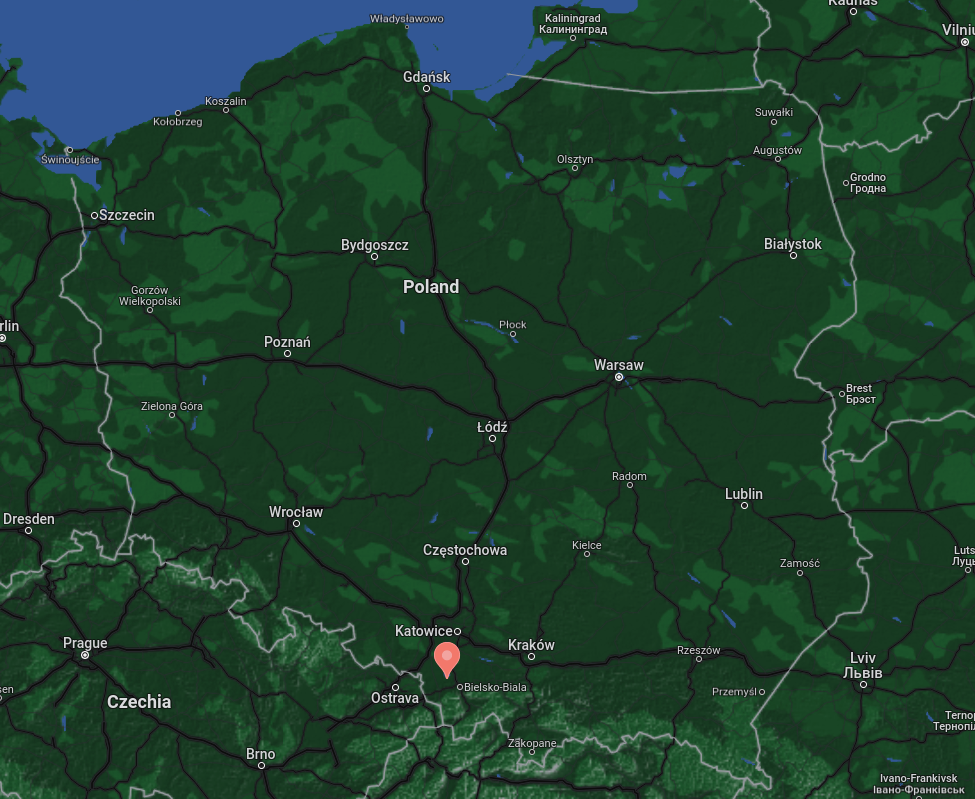
\includegraphics[width=\textwidth]{images/map.png}
    \caption{Lokalizacja, dla której wybrane zostały dane pogodowe}
    \label{map}
\end{figure}

Najważniejsze statystyki zbioru danych zostały także przedstawione w tabeli 
nr \ref{statystyki-danych}.

\begin{table}[H]
    \centering
    \caption{Statystyki zbioru danych} \label{statystyki-danych}
    \bigskip
    \begin{tabular}{|p{2cm}|p{2cm}p{2cm}p{2cm}p{2cm}|}
    \hline\xrowht[()]{.6cm}
    Zmienna & Średnia & Min & Max & Std \\
    \hline
    \hline\xrowht[()]{.6cm}
    u10 [$m\over{s}$] & 1.11 & -6.94 & 10.15 & 2.64\\
    \hline\xrowht[()]{.6cm}
    v10 [$m\over{s}$] & 1.28 & -9.02 & 10.70 & 2.77\\
    \hline\xrowht[()]{.6cm}
    t2m [K] & 271.4 & 247.8 & 285.7 & 5.8\\
    \hline\xrowht[()]{.6cm}
    e [m] & -1.16E-5 & -1.88E-4 & 4.78E-5 & 1.78E-5\\
    \hline\xrowht[()]{.6cm}
    ro [m] & 2E-5 & 3E-6 & 3.74E-4 & 1.4E-5\\
    \hline\xrowht[()]{.6cm}
    ssr [$J\over m^2$] & 8.51E4 & -3.12E-2 & 1.05E6 & 1.66E5\\
    \hline\xrowht[()]{.6cm}
    str [$J\over m^2$] & -1.28E5 & -4.17E5 & 3.20E4 & 8.64E4\\
    \hline\xrowht[()]{.6cm}
    sp [Pa] & 9.73E4 & 9.33E4 & 9.99E4 & 995\\
    \hline\xrowht[()]{.6cm}
    tp [m] & 9.77E-5 & 0 & 2.51E-3 & 1.95E-4\\

    \hline
    \end{tabular}
    \end{table}

% Data preprocessing: Describe the steps you took to clean and prepare 
% the data for analysis, such as removing duplicates, filling in missing 
% values, and standardizing units. This is an important step in ensuring 
% the quality and reliability of your results.
\subsection{Preprocessing}

W ramach preprocessingu wszystkie braki w danych zostały uzupełnione poprzez 
interpolację danej zmiennej w szeregu czasowym. Co więcej, w celach dalszego
wykorzystania danych do treningu algorytmów uczenia maszynowego zmienne zostały 
przeskalowane do przedziału [0, 1], co zapobiega stronniczości modeli ze względu
na typ parametru. Wszystkie zmienne są typu ilościowego i dalsza obróbka nie była
potrzebna.

% Data analysis: Explain the methods you used to analyze the data, 
% including any statistical techniques, machine learning algorithms, 
% or other models. Discuss the performance of these models and any 
% limitations or challenges you encountered.
\subsection{Analiza danych}

Autokorelacja jest narzędziem specyfikującym występowanie wzorców w danych. Jest ona 
opisana jako wartość korelacji dyskretnego szeregu czasowego względem tego samego sygnału
przesuniętego o zadane opóźnienie. Przy pomocy autokorelacji można zauważyć w danych
występowanie cykli, oraz prędkość z jaką trend szeregu się zmienia.

\begin{figure}[H]
    \centering
    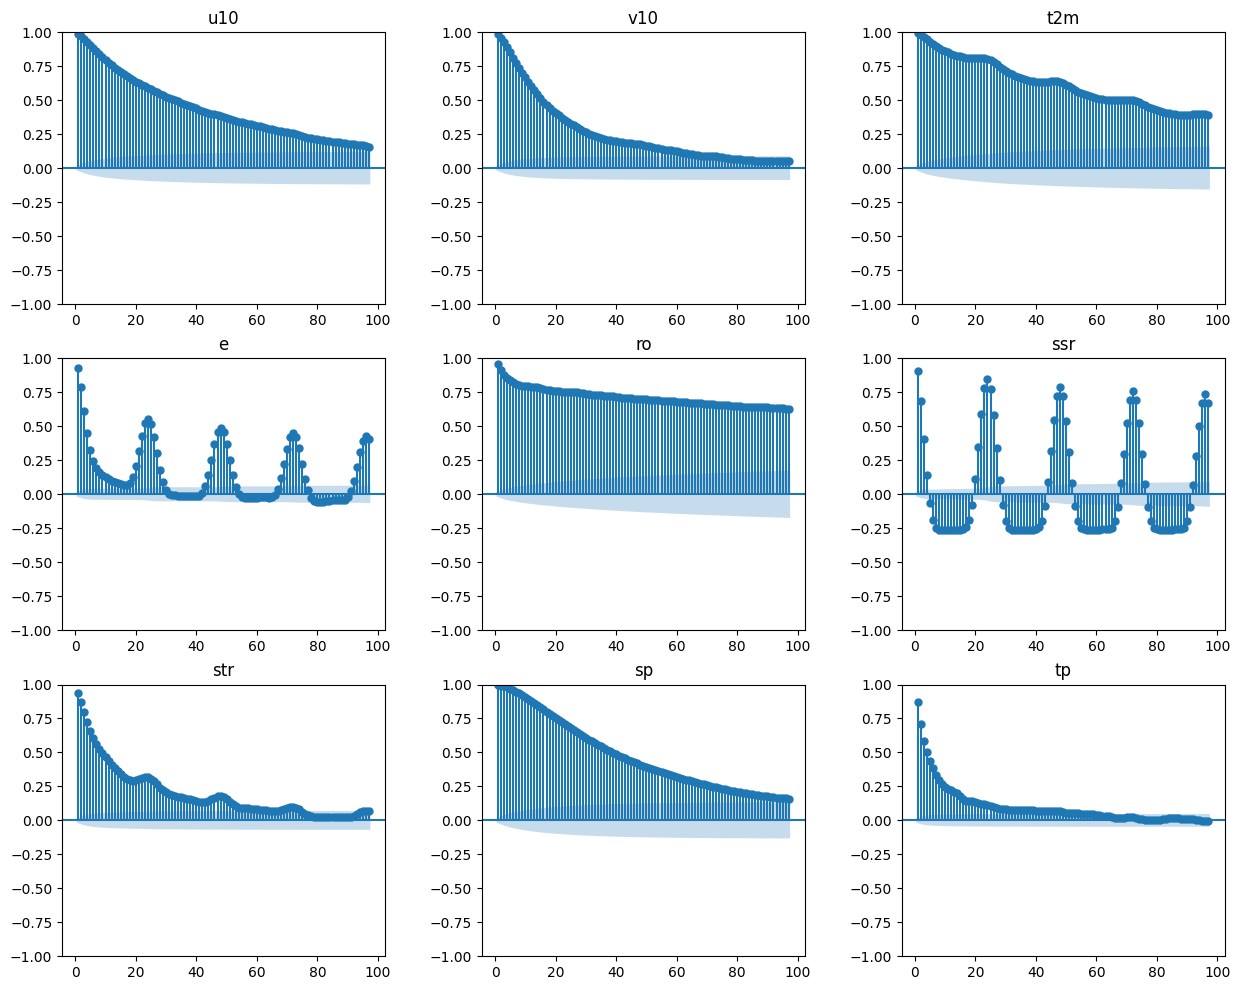
\includegraphics[width=\textwidth]{images/autocorrelation.png}
    \caption{Autokorelacja wybranych zmiennych względem opóźnienia o wartości od 
    1 godziny do 96 godzin.}
    \label{autocorrelation}
\end{figure}

Na rysunku \ref{autocorrelation} zaprezentowane zostały wykresy autokorelacji wybrenago
zbioru danych na przestrzeni 4 dni. Wyraźnie widać występowanie dziennych cykli i ich wpływ
na poszczególne pomiary. Wzrost wartości autokorelacji dla przesunięcia będącego
wielokrotnością doby jest widoczny dla temperatury, odparowania, promieniowania słonecznego i 
termicznego. Reszta zmiennych wykazuje stały spadek korelacji z rosnącym opóźnieniem. 
Szczególnie niskie wartości można zaobserwować dla opadów, dla których autokorelacja szyko spada
poniżej 0.2, co wskazuje na wyjątkowo chaotyczną naturę tego zjawiska.

Przy pomocy zebranych danych można także graficznie pokazać trajektorię zmian dla wybranych zminnych. Na rysunku \ref{temperature} widać zależność pomiędzy szeregiem czasowym temperatury
oraz kopią tego szeregu przesuniętą o 24 godziny. Wykres potwierdza wartość korelacji 
wskazaną na rysunku \ref{autocorrelation}. Gradient koloru widoczny na wykresie wskazuję
progresję wartości temperatury z czasem. Trajektoria dla pierwszych 9 dni jest pokazana 
na wykresie liniowym z prawej strony. 

\begin{figure}[H]
    \centering
    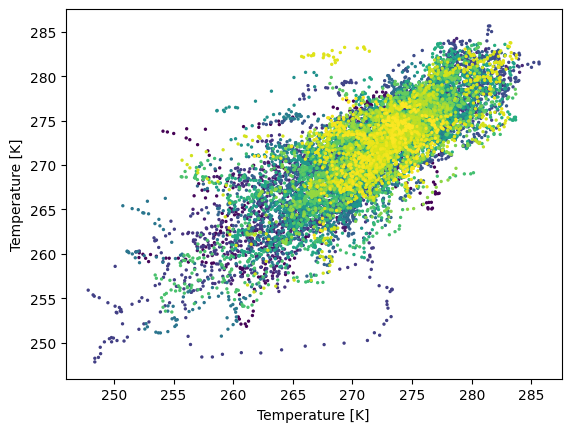
\includegraphics[width=0.45\textwidth]{images/temperature_scatter.png}
    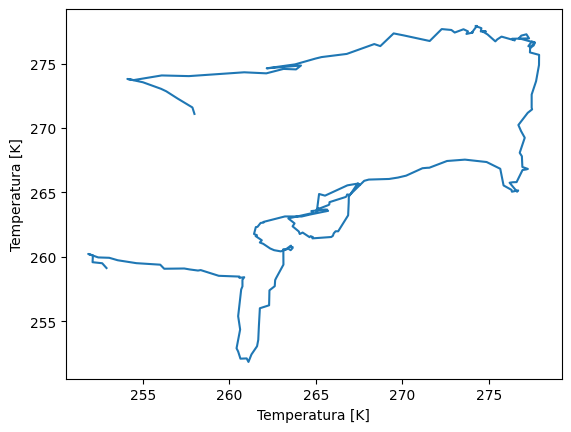
\includegraphics[width=0.45\textwidth]{images/temperature_line.png}
    \caption{Wykresy pokazujące relację pomiędzy wartościami temperatury, a tymi samymi 
    wartościami przesuniętymi w czasie o 24 godziny.}
    \label{temperature}
\end{figure}

Podobne zachowanie można także wyróżnić dla ciśnienia oraz reszty zmiennych wykazujących 
wysoką autokorelację. Jednak w przypadku opadów trajektoria dynamicznych zachowań systemu
staję się o wiele trudniejsza w śledzeniu, co zostału ukazane na rysunku \ref{pressure-precipitation} porównującym wykresy dla ciśnienia oraz opadów. 

% \begin{figure}[H]
%     \centering
%     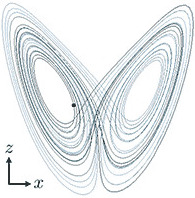
\includegraphics[width=0.5\textwidth]{images/lorenz.jpeg}
%     \caption{caption}
%     \label{line}
% \end{figure}

\begin{figure}[H]
    \centering
    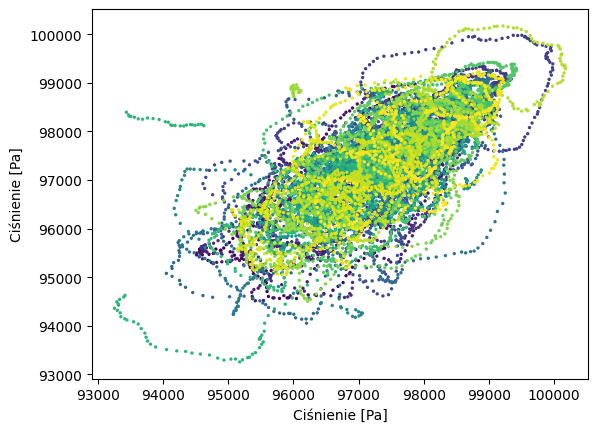
\includegraphics[width=0.45\textwidth]{images/pressure_scatter.png}
    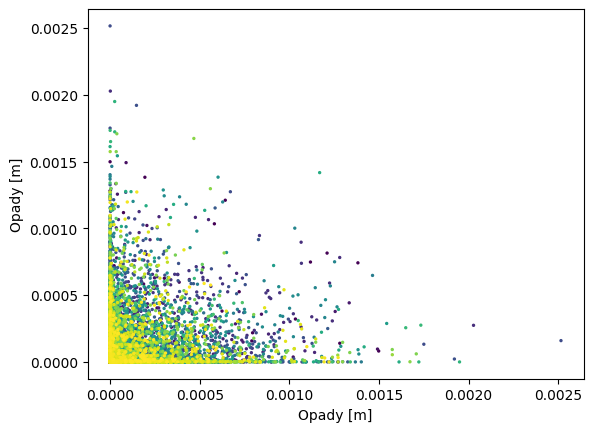
\includegraphics[width=0.45\textwidth]{images/precipitation_scatter.png}
    \caption{Zależność ciśnienia (z lewej) oraz opadów (z prawej) względem 
    swoich przesuniętych kopii.}
    \label{pressure-precipitation}
\end{figure}

Wartości opadów zdają się bardzo mocno skoncentrowane wokół zera, z wieloma 
odbiegającymi obserwacjami. W szczególności widać dużo pomiarów w pobliżu 
osi x i y, co wskazuję na znaczącą ilość pomiarów oznaczających nagły wzrost opadów
po okresie bez opadów, oraz gwałtowne zaprzestanie opadów.

W celu pokazania dystrybucji zmiennych względem ich opóźnionych szeregów, na następującym 
wykresie \ref{hex} pokazana została koncentracja pomiarów o wskazanych wartościach.

\begin{figure}[H]
    \centering
    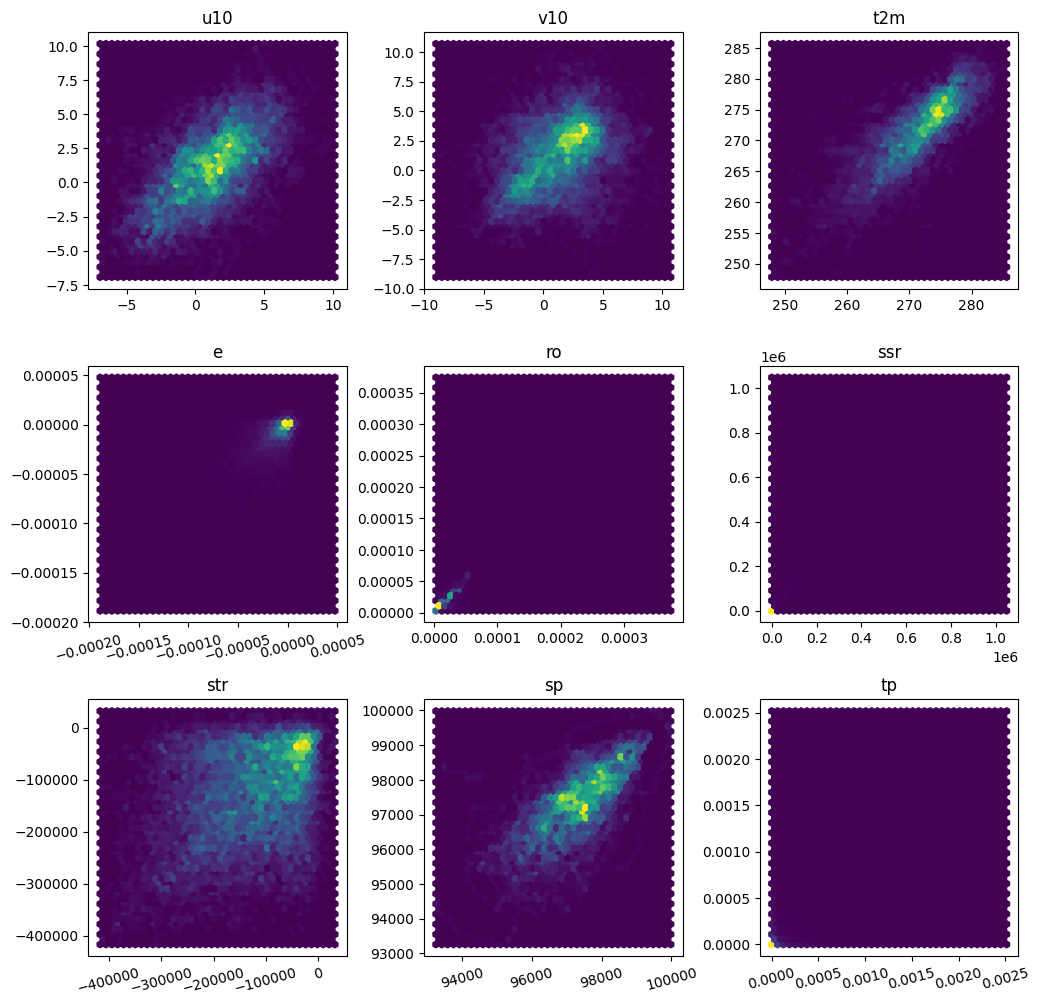
\includegraphics[width=\textwidth]{images/autocorrelation_hex.png}
    \caption{Dystrybucja pomiarów na wykresie względem orginalnego szeregu czasowego,
    oraz szeregu przesuniętego o 24 godziny.}
    \label{hex}
\end{figure}

Na powyższym wykresie \ref{hex} widać duży zakres zmienności promieniowania termicznego
który jest niezależny od wcześniej zarejestrowanych pomiarów. Z kolei bardzo mała wariancja 
została zaobserwowana dla odpływów wody, promieniowania słonecznego i opadów, które wskazują 
jedynie periodyczne odchylenia od zera. W przypadku prędkości wiatru, temperatury oraz 
ciśnienia widoczna jest wysoka autokorelacja, które została już wcześniej odnotowana. 

Duże wartości autokorelacji są dobrym znakiem wskazującym na możliwości przewidywania przyszłych
obserwacji jedynie na podstawie obserwacji już zarejestrowanych. W przypadku reszty zmiennych
potrzebna jest analiza ze względu na korelację pomiędzy parami parametrów obserwacji, w 
poszukiwaniu dodatkowych zależności.

Na następującym rysunku \ref{matrix} została ukazana wartość korelacji pomiędzy wszystkimi 
parami zmiennych. W wielu przypadkach odnotowane wartości są dość małe, co wskazuje na brak
bezpośrednich zależności jednej zmiennej na drugą zmienną. 

\begin{figure}[H]
    \centering
    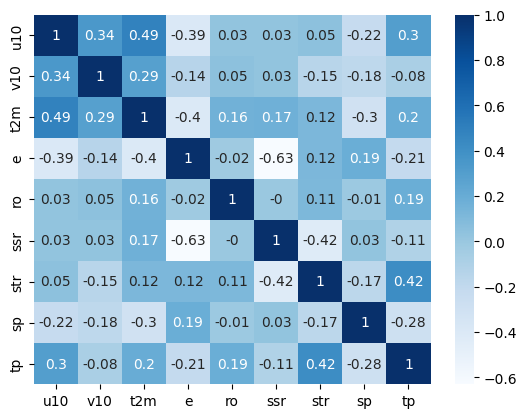
\includegraphics[width=\textwidth]{images/correlation_matrix.png}
    \caption{Macierz korelacji parametrów}
    \label{matrix}
\end{figure}

Wyjątkiem na powyższym wykresie jest zależność pomiędzy odparowaniem oraz promieniowaniem 
słonecznym wskazująca na ujemną korelację. Ponieważ z przyjętej konwencji ujemna ewaporacja
wskazuję na parowanie wody, ta zależność okazuję się trywialna. 

Brak dalszych korelacji w danych jest dobrą oznaką sygnalizującą brak redundancji danych.
Niestety oznacza to także że najprawdopodobniej cały zakres parametrów musi być przeanalizowany
w celu znalezienia szukanych zależności i stworzenia modelu prognozującego. 

W celu dalszej analizy dostępnych danych stworzone zostały wykresy Q-Q, pokazujące normalność
dystrybucji danych. Wykresy te zostały pokazane na rysunku \ref{qq}. Proste linie dla prędkości 
wiatru sygnalizują normalność dystrybucji. Pozostałe parametry pomimo bliskiego odwzorowania
dystrybucji normalnej, posiadają inną charakterystykę. 


\begin{figure}[H]
    \centering
    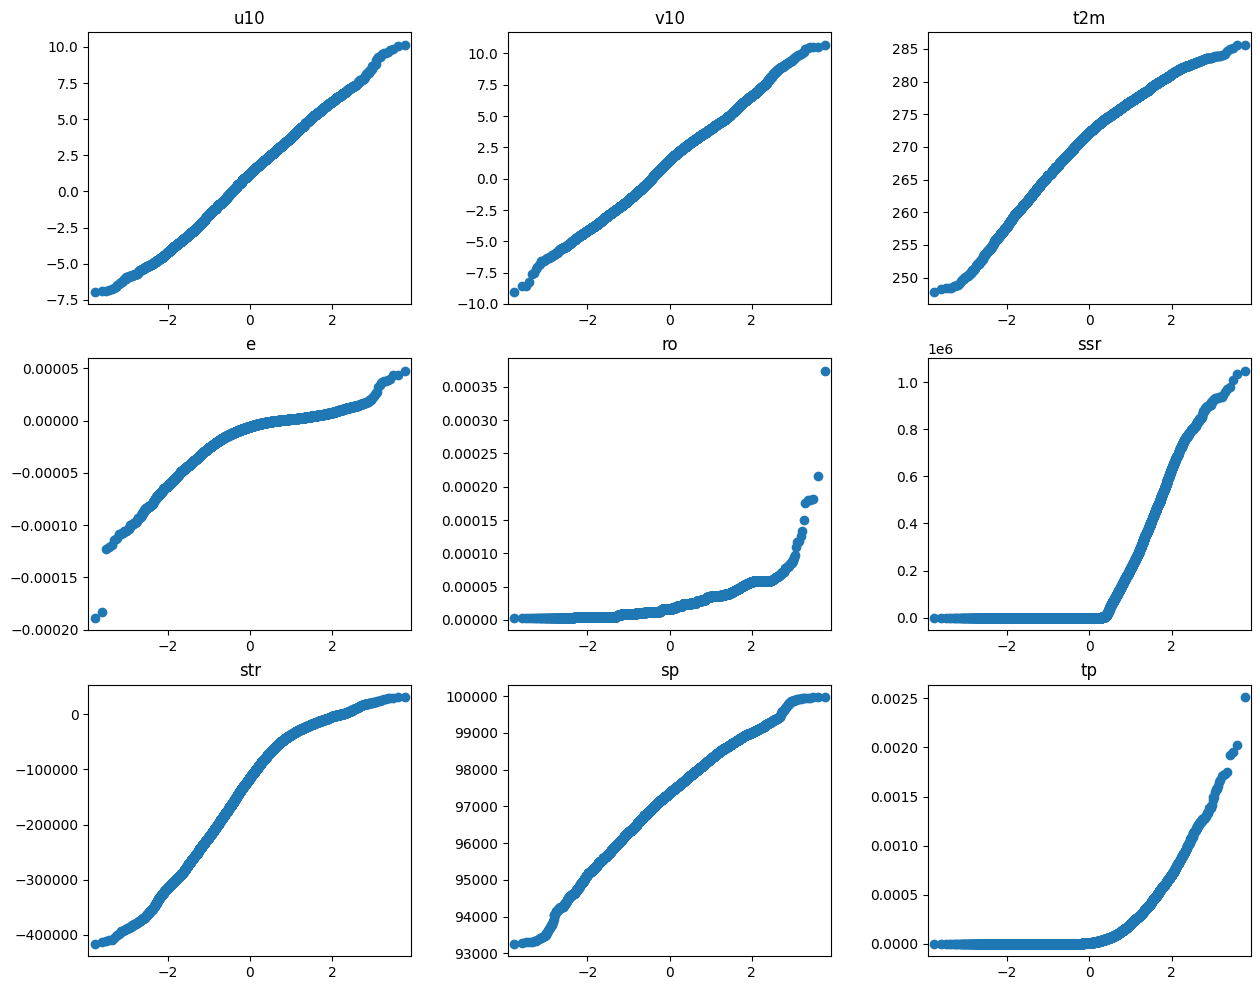
\includegraphics[width=\textwidth]{images/qq.png}
    \caption{Wykresy Q-Q}
    \label{qq}
\end{figure}

Na następującym rysunku \ref{box} pokazującym wykresy pudełkowe widać wartości medianę, pierwszy i trzeci
kwartyl danych oraz wartości odstające. 

\begin{figure}[H]
    \centering
    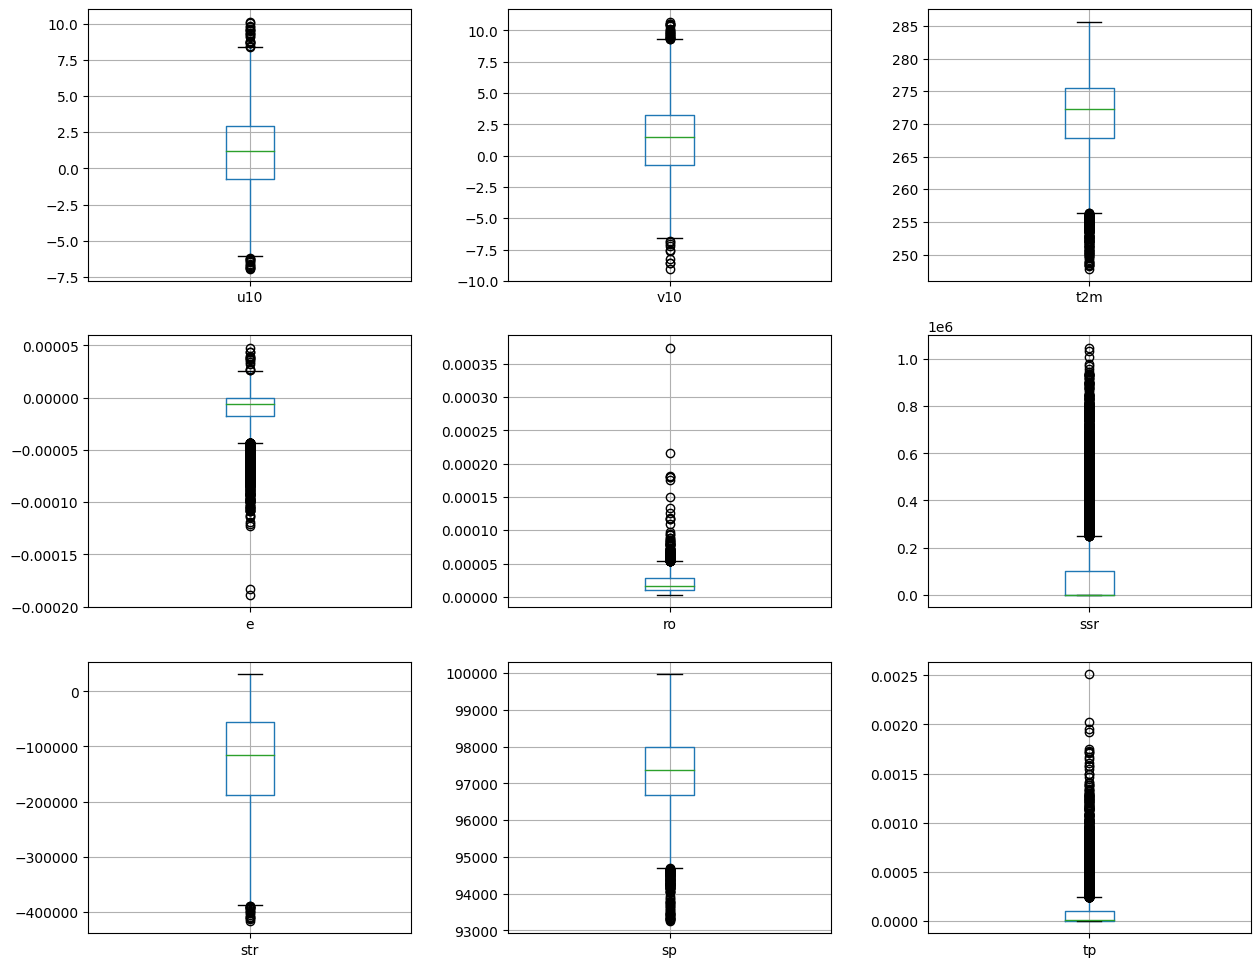
\includegraphics[width=\textwidth]{images/box.png}
    \caption{Wykresy pudełkowe wygenerowane dla poszczególnych atrybutów}
    \label{box}
\end{figure}

Z powyższych wykresów można wnioskować o znaczącej liczbie anomali dla wartości promieniowania słonecznego,
opadów oraz odparowania. Wartości odstające dla temperatury leżały wyłącznie po lewej stronie dystrybucji,
poniżej zaobserwowanych pomiarów. Anomalie wskazane tym sposobem wyróżniają pomiary będące poniżej $-18^\circ C$. Co więcej, ponownie można zaobserwować bardzo wąską dystrybucję opadów posiadającą dużo wartości znacznie
przewyższających wartość oczekiwaną. 

Na rysunku \ref{hist} pokazano histogramy ilustrujące rozkład danych. Potwierdzają one normalność dystrybucji
dla wartości prędkości wiatru. Pozostałe dystrybucje wykazują się pewną asymetrią, w której duża liczba 
obserwacji odbiega od centrum dystrybucji wyraźnie w jedną stronę. 

\begin{figure}[H]
    \centering
    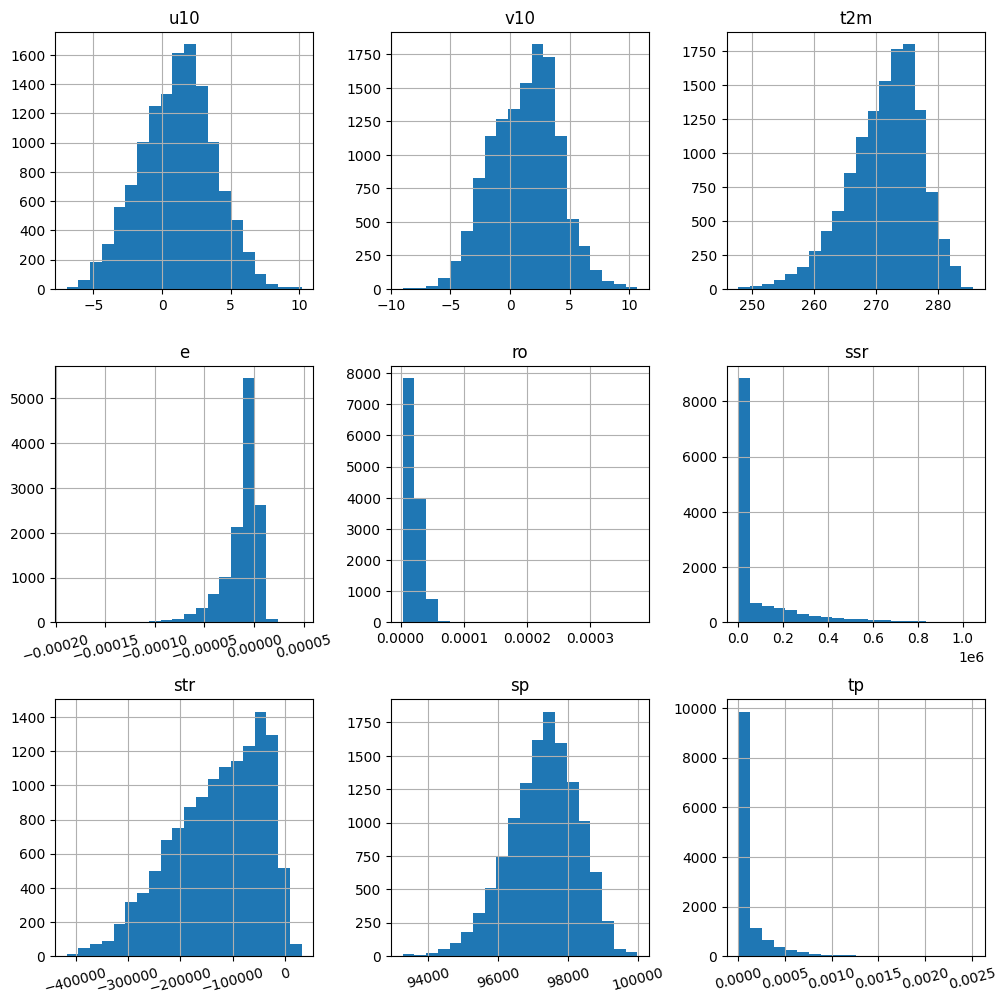
\includegraphics[width=\textwidth]{images/hist.png}
    \caption{Histogramy wygenerowane dla poszczególnych atrybutów}
    \label{hist}
\end{figure}

Ostatnią wizualizacją są wykresy pokazujące przebieg wartości szeregu czasowego w okresie 120 dni, z 
wartościami zakumulowanymi z czterech dni. Wykresy liniowe na rysunku \ref{line} pokazują zmienność
danych w czasie. Dla większości zmiennych widzimy charakter oscylacyjny. W przypadku promieniowania 
słonecznego zaobserwować można także dużą wariacje w danych nawet w małych przedziałach czasu. 
Dużym wyjątkiem od reszty zmiennych jest wartość odpływu wody, która nie ulega cyklicznym zmianom, lecz
wykazuje nagłe skoki w wartości i okresy stabilności.

\begin{figure}[H]
    \centering
    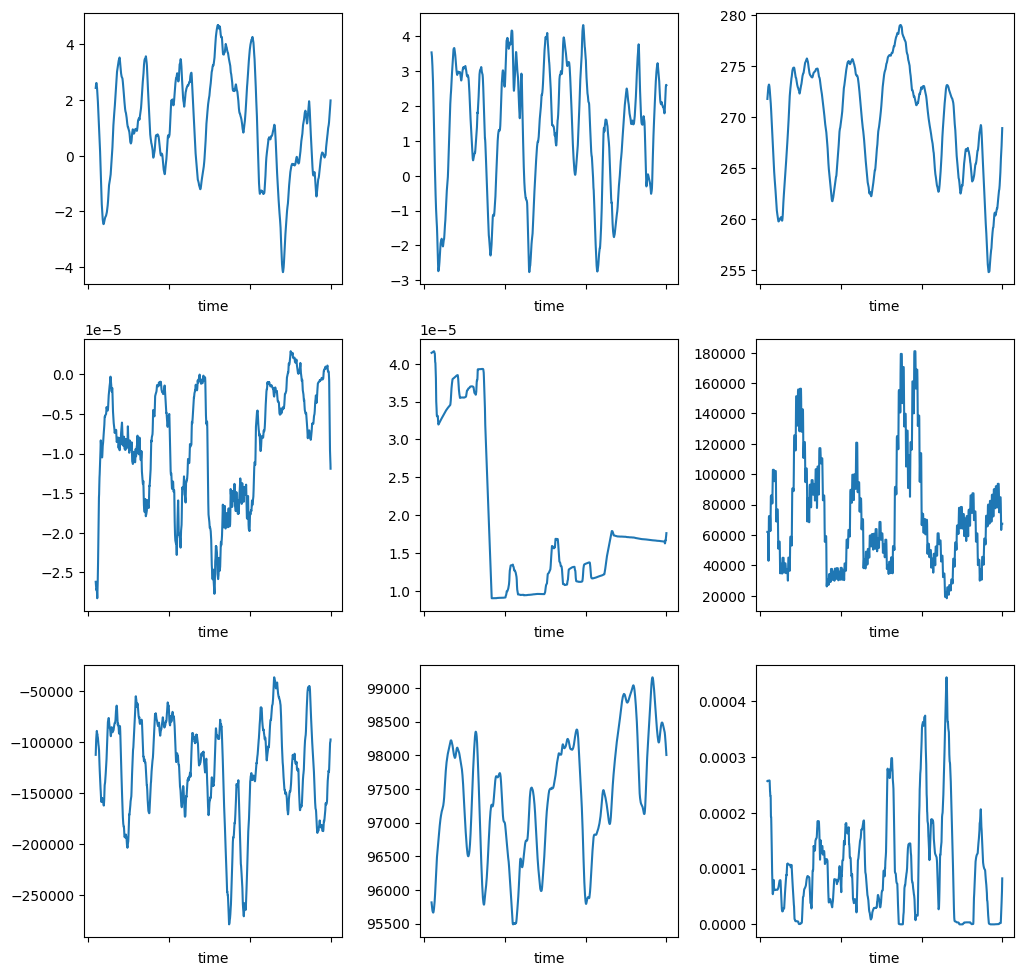
\includegraphics[width=\textwidth]{images/line.png}
    \caption{Wykresy liniowe pokazujące wartość średniej kroczącej z czterech dni na przestrzeni 120 dni}
    \label{line}
\end{figure}

Pokazane wykresy i przeprowadzona interpretacja wskazują na złożoność dostępnych danych
i możliwe problemy w ich analizie. Wysoka zmienność obserwacji w czasie oraz mało przewidywalna
charakterystyka, sprawiają że tworzenie dokładnych prognoz jest wyzwaniem. Co więcej, 
cykliczność zaobserwowana wśród niektórych zmiennych może sprawiać wyzwanie dla niektórych
metod uczenia maszynowego, które nie radzą sobie z danymi o dużej częstotliwości zmian. 

Przeprowadzona analiza była jednak tylko wstępem do dalszych badań i wykazuje ograniczone
możliwości metod czysto statystycznych w modelowaniu pogody.